\documentclass[11pt]{article}
\usepackage[margin=1in]{geometry}
\usepackage{amsthm, amsmath, amssymb, mathtools}
\usepackage{graphicx}
\usepackage{placeins}
\usepackage{setspace}
\usepackage{booktabs}
\usepackage{subcaption}
\usepackage{hyperref}

\title{DOT Project Data Summary}

\begin{document}
\maketitle

This document describes the three data sources available for this project. The goal of this
project is to add job complexity information to the 1940 US Census. The available data are
all the editions of the Dictionary of Occupational Titles (DOT), the 1940 US Census, and
the 1940 Census Alphabetical Index of Jobs.

\section{Dictionary of Occupational Titles}

The DOT provides job descriptions for thousands of jobs and was meant to be used as a tool for matching job seekers to jobs. The descriptions include information regarding the industry and occupation group the job is in. There are 5 editions of the DOT: 1939, 1949, 1965, 1977, and 1991. Each edition has about 30,000 job titles and 20,000 definitions (one definition can correspond to multiple job titles). Starting with the 1965 edition, the job codes include 3 digits that describe the job complexity with regards to data, people, and things.

\begin{figure}[h]
    \centering
    \caption{Example definition from the 1939 DOT}
    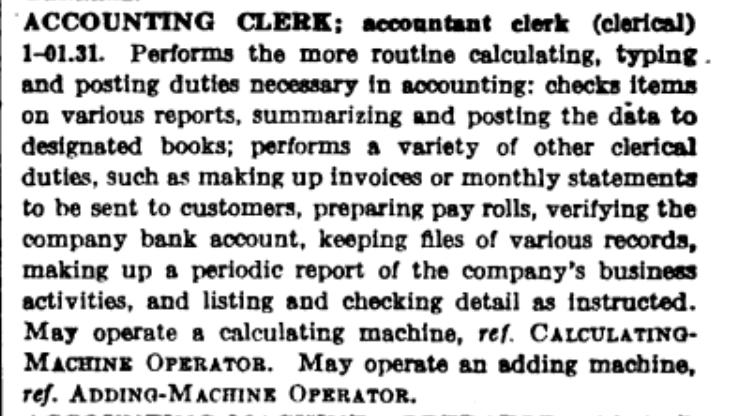
\includegraphics[width=0.6\textwidth, keepaspectratio=true]{dot_def}
\end{figure}

\begin{figure}[h]
        \centering
        \caption{Explanation of Data, People, Things Code}
        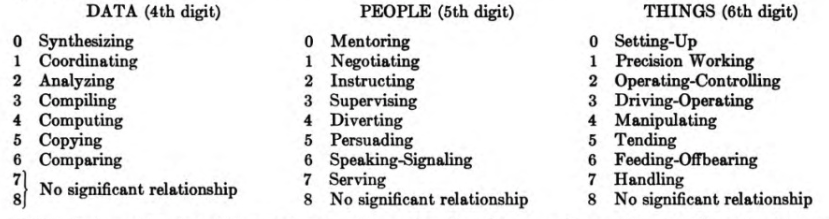
\includegraphics[width=0.95\textwidth, keepaspectratio=true]{DPT}
\end{figure}

\FloatBarrier

\section{1940 US Census}

The United States conducts a census every ten years to collect data about its population. The Census collects a wide range of information about respondents including occupation, income, education, and place of residence. The data is confidential, but becomes publicly available 72 years after Census Day. The data from the 1940 Census became publicly available in April of 2012.

In the 1940 census, every respondent listed their occupation. These occupation names are not standardized and contain many misspellings. In addition to each person's reported occupation, we also have their designated Census occupation code. There are about 400 census occupation codes, and they correspond to coarse categories such as lawyer or manager. The occupation codes and their corresponding categories can be seen \href{https://usa.ipums.org/usa/volii/occ1940.shtml}{here}. The census contains around 130 million observations. We instead work with a file that contains the number of observations for every combination of occupation title and census code.

\section{1940 Census Alphabetical List of Titles}

In every census, the US Census Board creates a list of official job titles and their corresponding census occupation codes and industry. Census employees would use this list to map each respondent's listed title to a census occupation code. This list contains about 12,000 job titles.

\section{Current Approach}

Our current approach has been to match job titles in the 1940 census to job titles in the 1940 census alphabetical index of titles based on exact matches in the occupation code and exact/inexact matches in the job title. We then plan to match job titles in the DOT to job titles in the alphabetical index. We assume this will be slightly easier since both data sources contain minimal misspellings, as opposed to the 1940 census.


\end{document}
